%==================== TITLE SLIDE ====================
{
\setbeamertemplate{footline}{}
\begin{frame}[noframenumbering]

\vspace{1.6cm}

\begin{center}
    {\fontsize{24}{28}\selectfont \color{tugreen}
    Case Study II: \\[0.3cm]
    Styrian Health Data}
\end{center}

\vspace{0.4cm}

\begin{center}
    {\large Week 5 Update: Spatial analysis and Model Improvements}
\end{center}

\vspace{0.3cm}

\begin{flushleft}
    {\normalsize
    Rohith B Chowdappa\\
    Nixon M Paulson\\
    Maria Cherian}
\end{flushleft}

\end{frame}
}

\begin{frame}{Study Overview \& Objectives}

\textbf{Study Focus:}
\begin{itemize}
    \item This study applies spatial analysis to patient-level BP data across Austria to uncover geographic patterns.
\end{itemize}

\textbf{Research Questions:}
\begin{enumerate}
    \item Does \textbf{blood pressure vary} by \textbf{urban-rural typology}?
    \item Is there \textbf{spatial clustering of hypertension} across districts?
    \item Does \textbf{regional GDP (NUTS3)} correlate with \textbf{blood pressure levels}?
\end{enumerate}

\end{frame}

%==================== Next Slide: Data ====================
\begin{frame}{Data Sources}

\begin{itemize}
    \item Patient-level \textbf{BP records} linked to Austrian administrative geography (\textbf{Bezirk/NUTS3})
    \item Open-source regional indicators from \url{https://www.statistik.at/atlas/}
    \begin{itemize}
        \item Gross Domestic Product per Capita - NUTS3
        \item Divisions according to urban and rural areas
    \end{itemize}
\end{itemize}

\end{frame}


\begin{frame}{Data Limitations}

\small

\begin{itemize}

\item \textbf{Urban--Rural match rate:} Municipality-level matching performed using the Eurostat urban--rural typology CSV.

\item Some \textit{Gemeinden} could not be matched directly due to post-2015 Austrian municipal mergers 
(e.g., Bruck an der Mur + Mürzzuschlag $\rightarrow$ Bruck-Mürzzuschlag; 
Hartberg + Fürstenfeld $\rightarrow$ Hartberg-Fürstenfeld).

\item \textbf{Patient threshold:} Only districts and NUTS3 regions with $\geq 30$ patients were retained for spatial and GDP-related analyses.

\item Grey districts/regions on maps indicate missing data:
either no patients recorded in that area or unresolved municipality matching.

\end{itemize}

\end{frame}

\begin{frame}{Module 1 --- Urban-Rural Typology}

\begin{itemize}
    \item Patients matched to Eurostat urban-rural typology (\textit{Gemeinde} level)
    
    \item Five tiers:
    Urban Core, Intermediate, Peri-urban, Rural, Remote Rural
    
    \item District classification based on modal urban-rural tier
    
    \item Hypertension:
    \[
    \text{SBP} \geq 140 \text{ mmHg}
    \]
    
    \item Spatial weights: Queen contiguity (row-standardised)
    
    \item Spatial tests:
    Moran's I and LISA
\end{itemize}

\end{frame}

\begin{frame}{Urban-Rural Typology vs Hypertension}
\centering
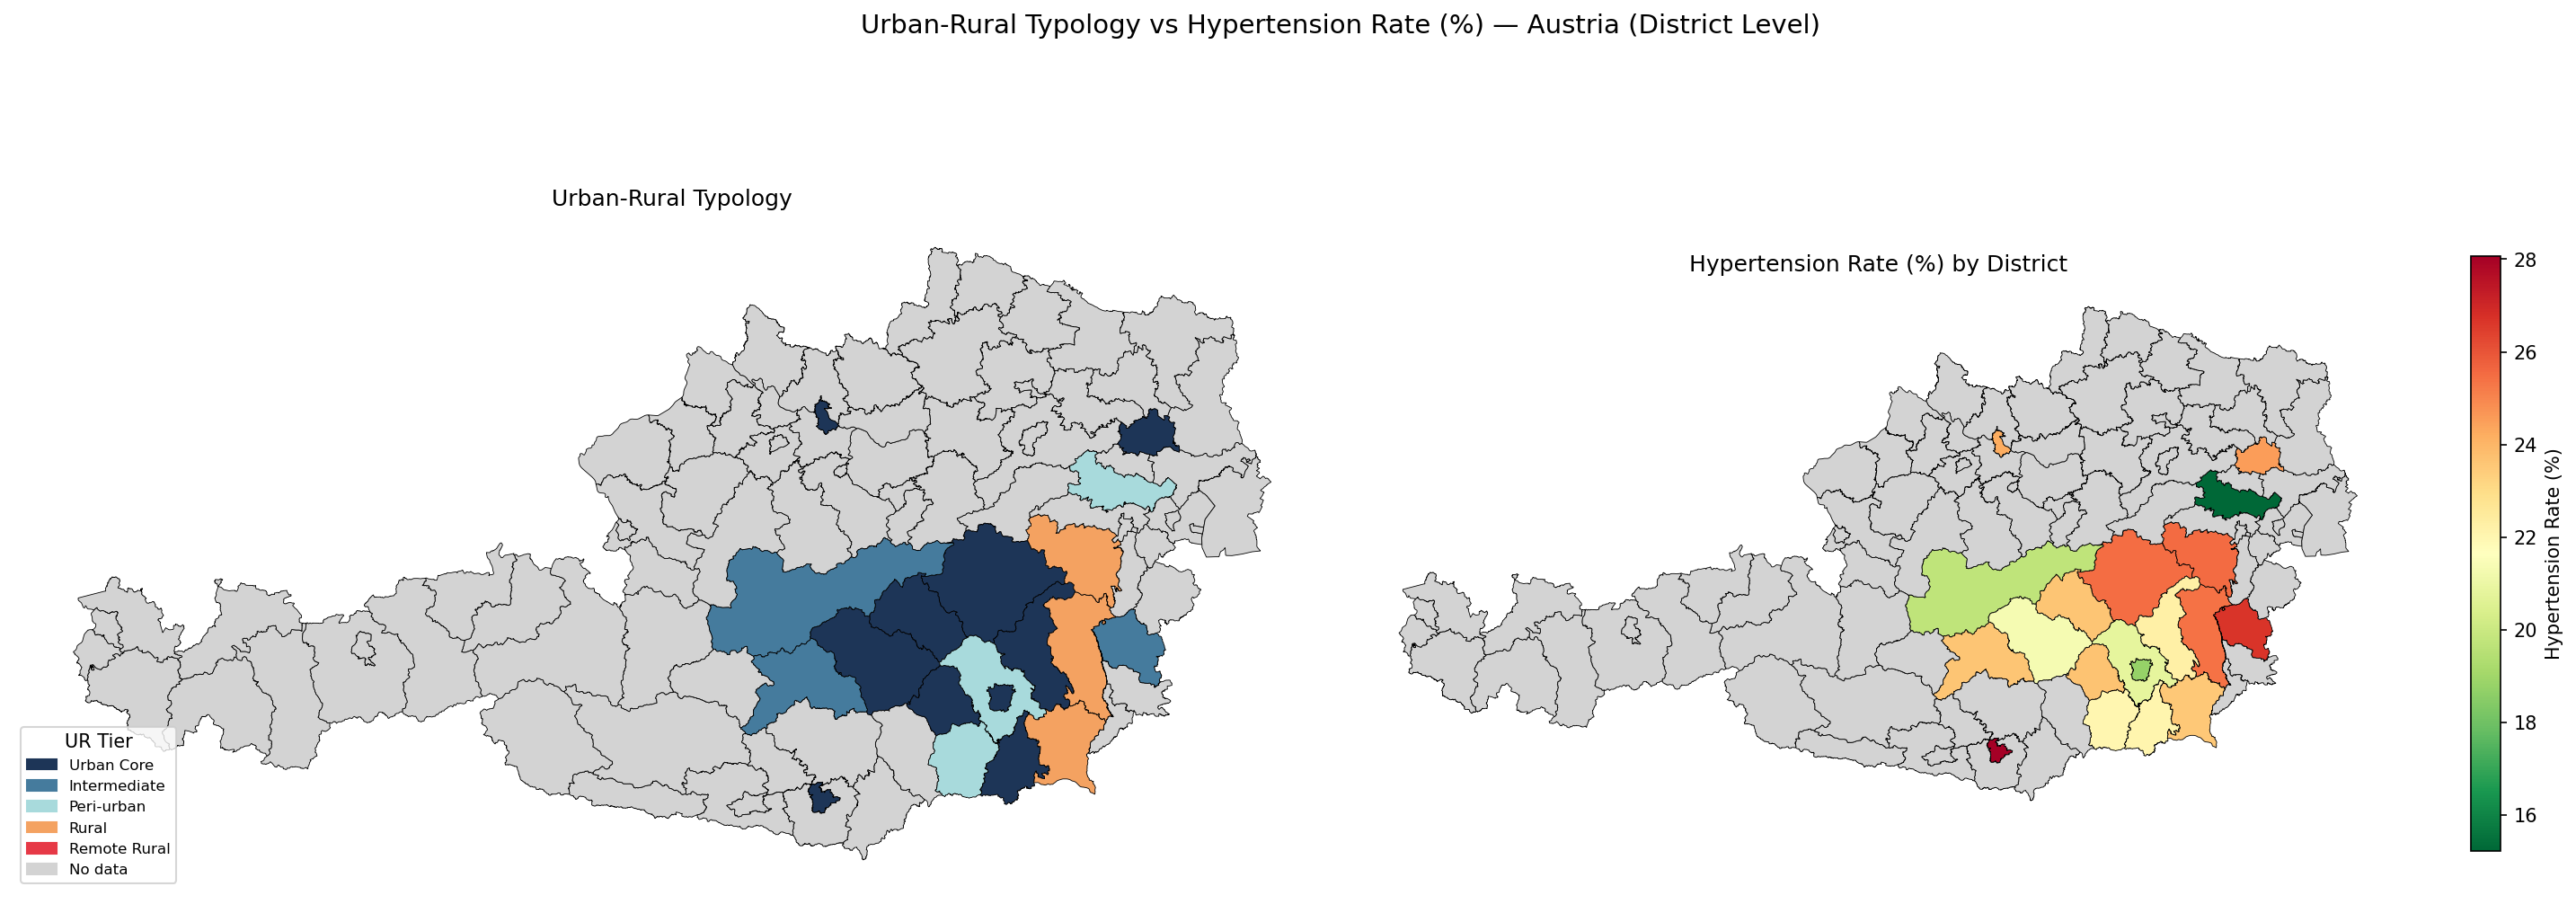
\includegraphics[width=0.9\linewidth, height=0.9\textheight, keepaspectratio]{figures/map_ur_vs_hyp_district.png}
\end{frame}

\begin{frame}{Urban-Rural Typology vs Mean Diastolic BP}
\centering
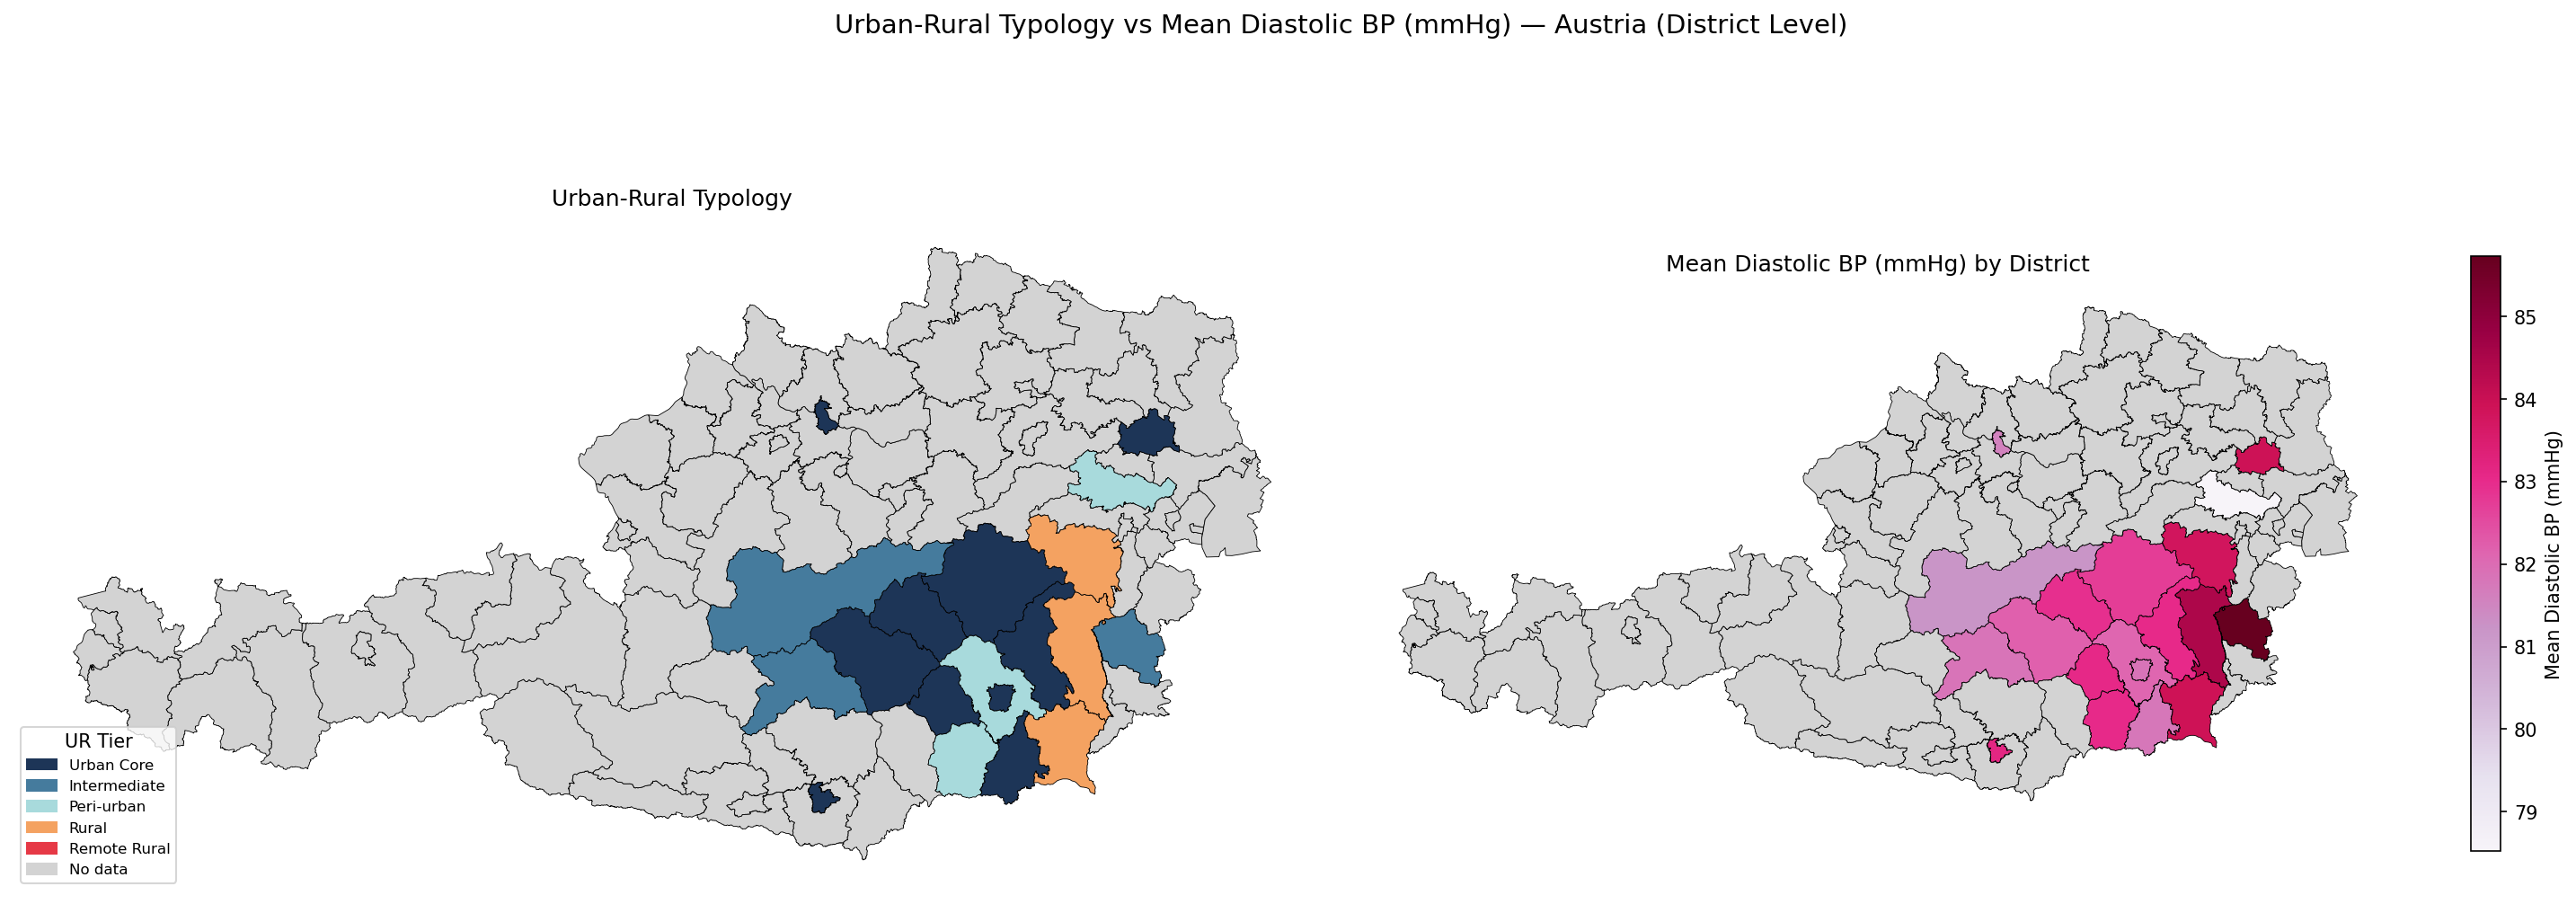
\includegraphics[width=0.9\linewidth, height=0.9\textheight, keepaspectratio]{figures/map_ur_vs_diabp_district.png}
\end{frame}

\begin{frame}{Urban-Rural Typology vs Mean Systolic BP}
\centering
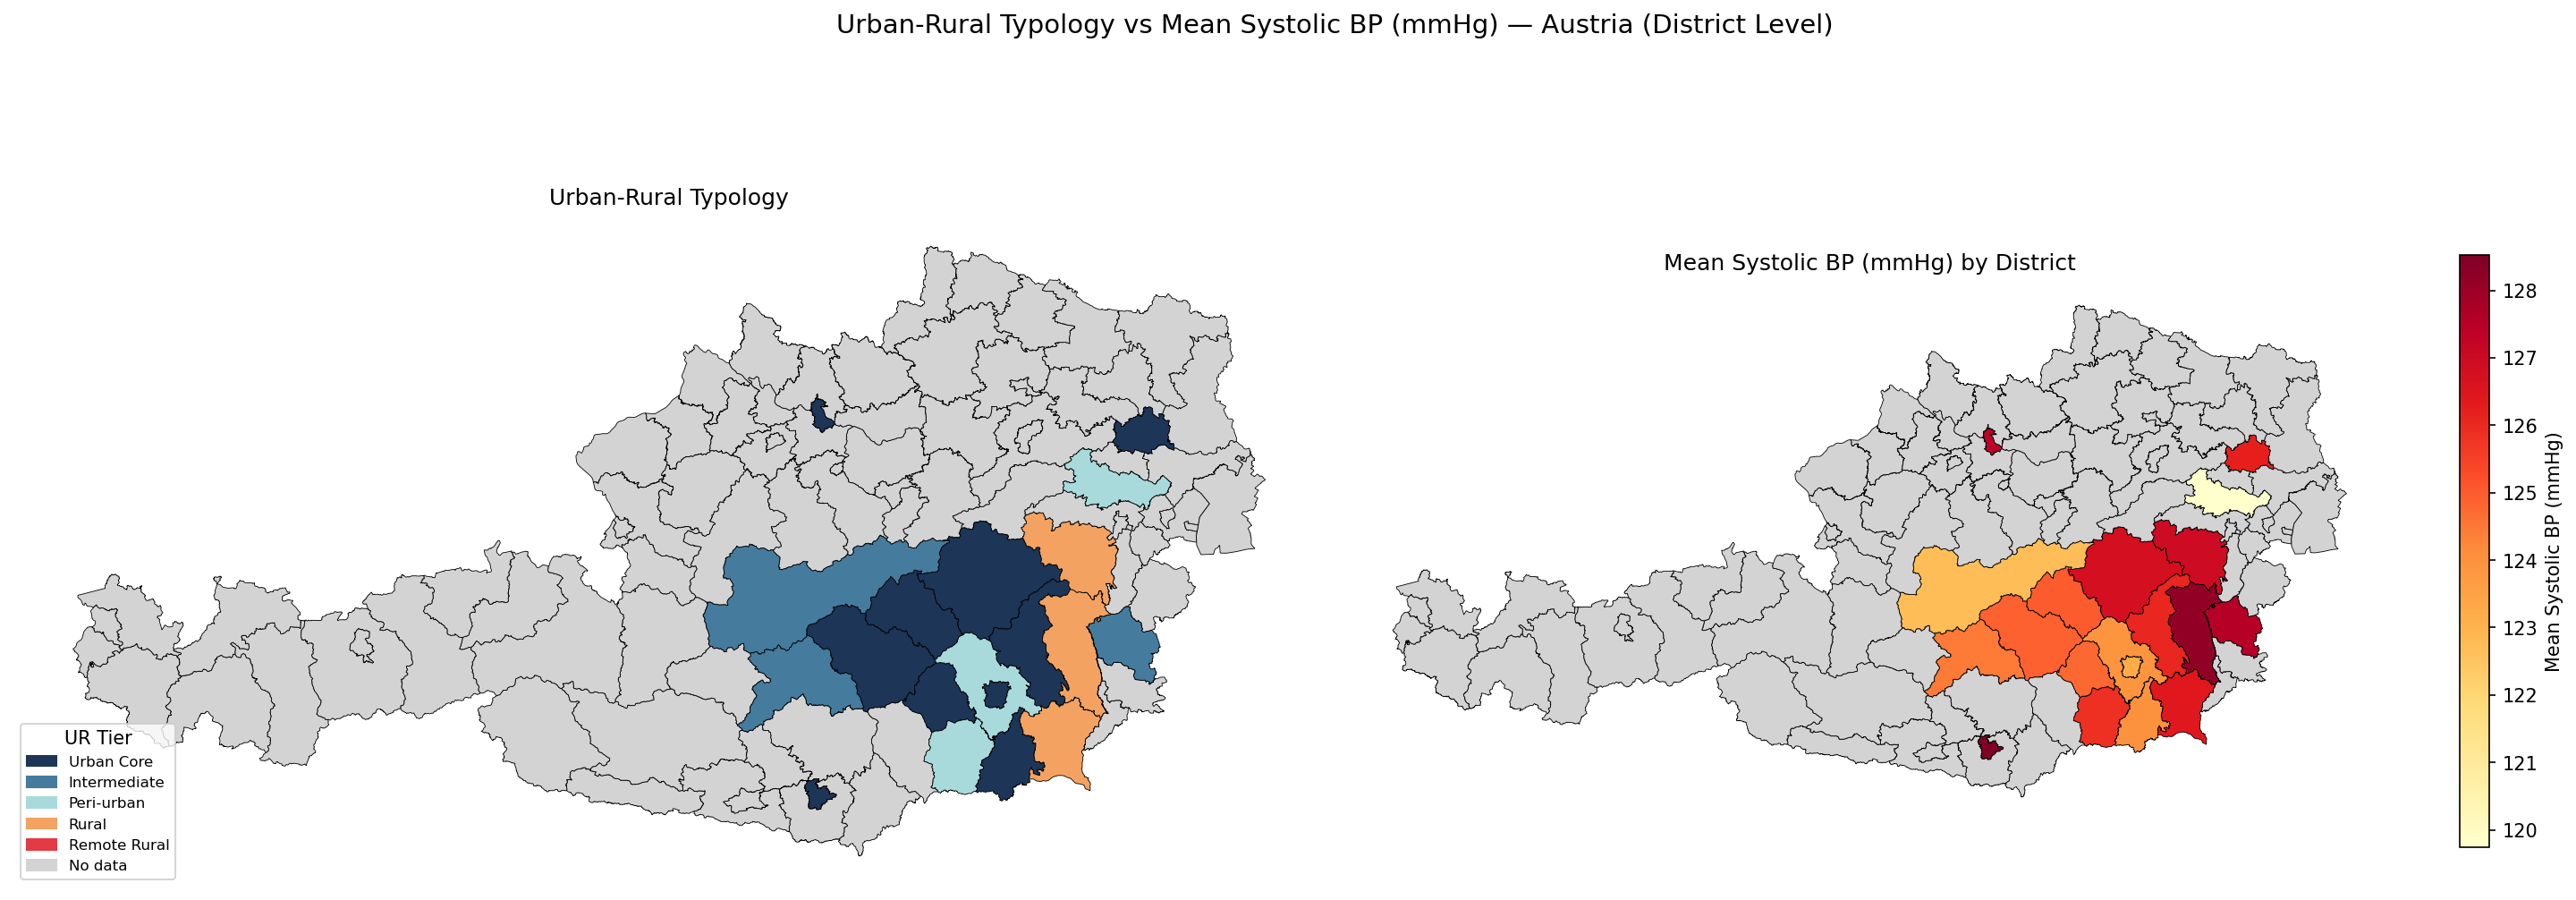
\includegraphics[width=0.9\linewidth, height=0.9\textheight, keepaspectratio]{figures/map_ur_vs_sysbp_district.png}
\end{frame}

\begin{frame}{Spatial Autocorrelation Analysis (Moran’s I)}
\centering
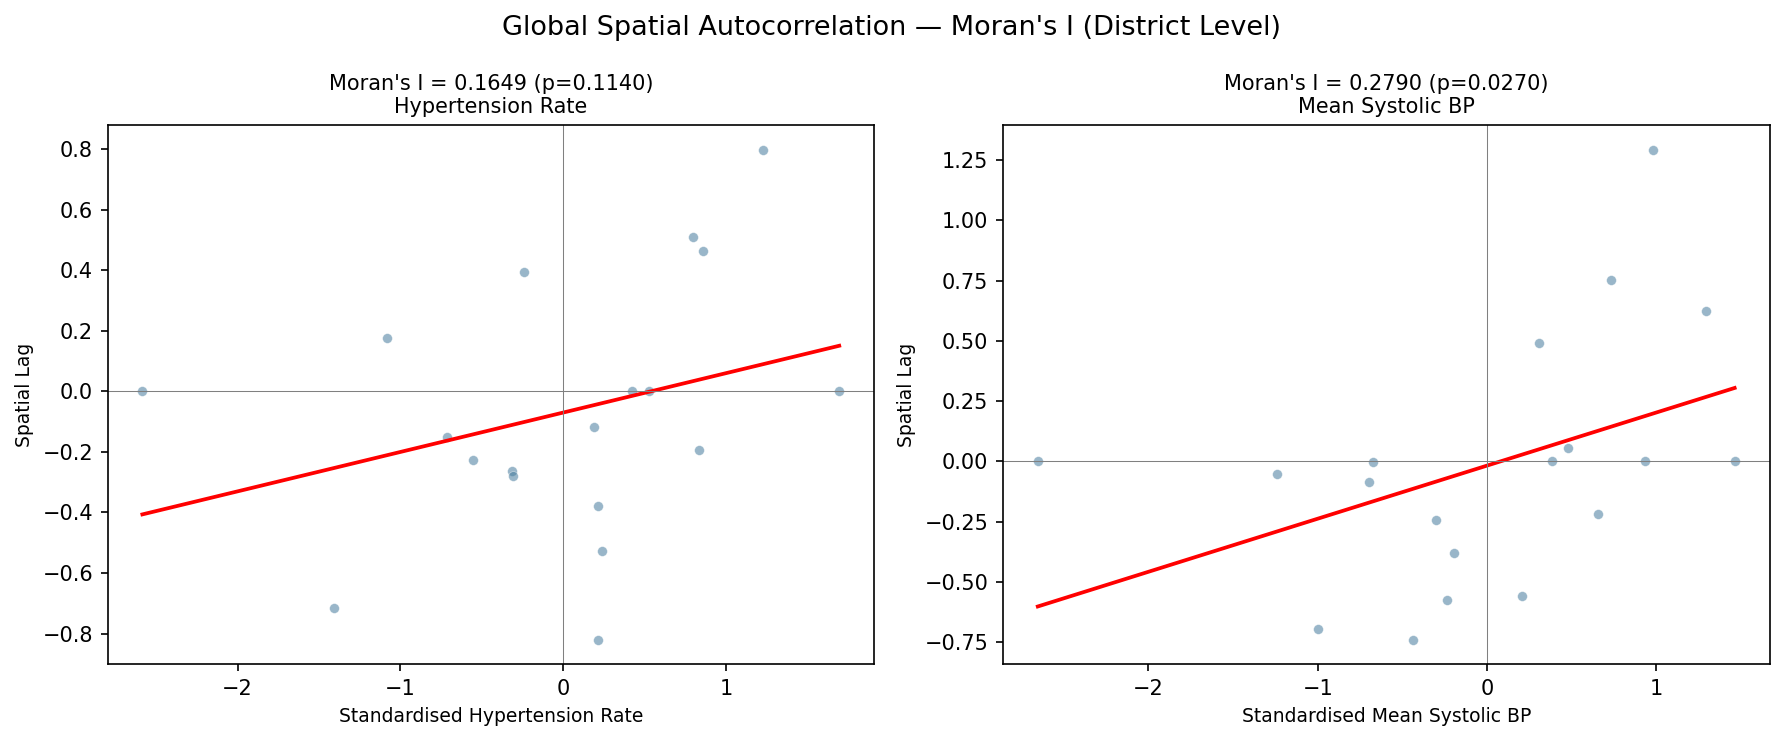
\includegraphics[width=0.9\linewidth, height=0.9\textheight, keepaspectratio]{figures/morans_I_district.png}
\end{frame}


\begin{frame}
\small
\begin{itemize}
    \item Urban--rural typology alone does not explain the spatial pattern.
    
    \item Higher systolic BP, diastolic BP, and hypertension prevalence are concentrated in eastern and southeastern Austrian districts.
    \item Elevated rates occurred across urban, intermediate, and rural districts
    \item Neighboring districts tend to show similar cardiovascular risk profiles, indicating spatial clustering.
    
    % \item Moran’s I confirms significant positive spatial autocorrelation for hypertension prevalence ($I = 0.154$, $p = 0.025$).
\end{itemize}

\end{frame}


\begin{frame}{LISA Cluster Findings (District Level)}
\centering
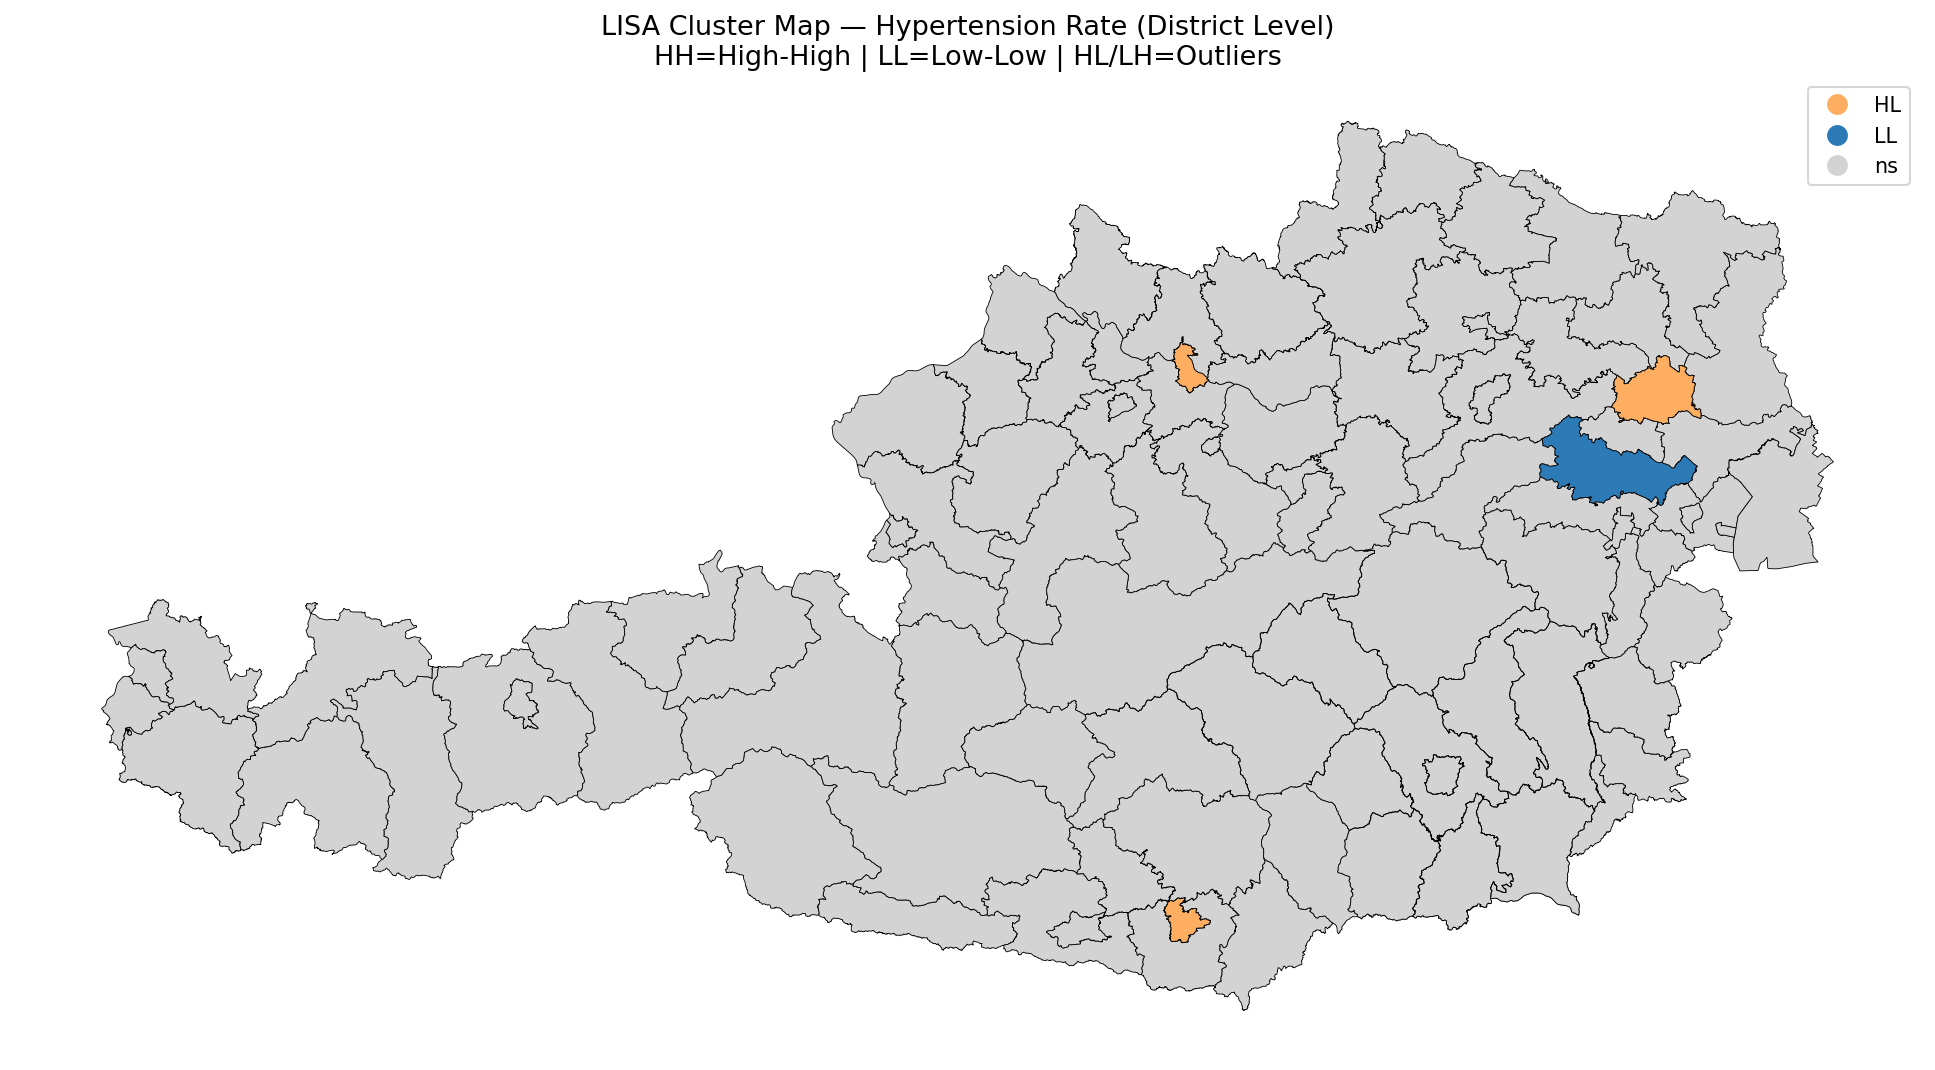
\includegraphics[width=0.9\linewidth, height=0.9\textheight, keepaspectratio]{figures/lisa_clusters_hyp_district.png}
\end{frame}

\begin{frame}{LISA Cluster Findings (District Level)}
\centering
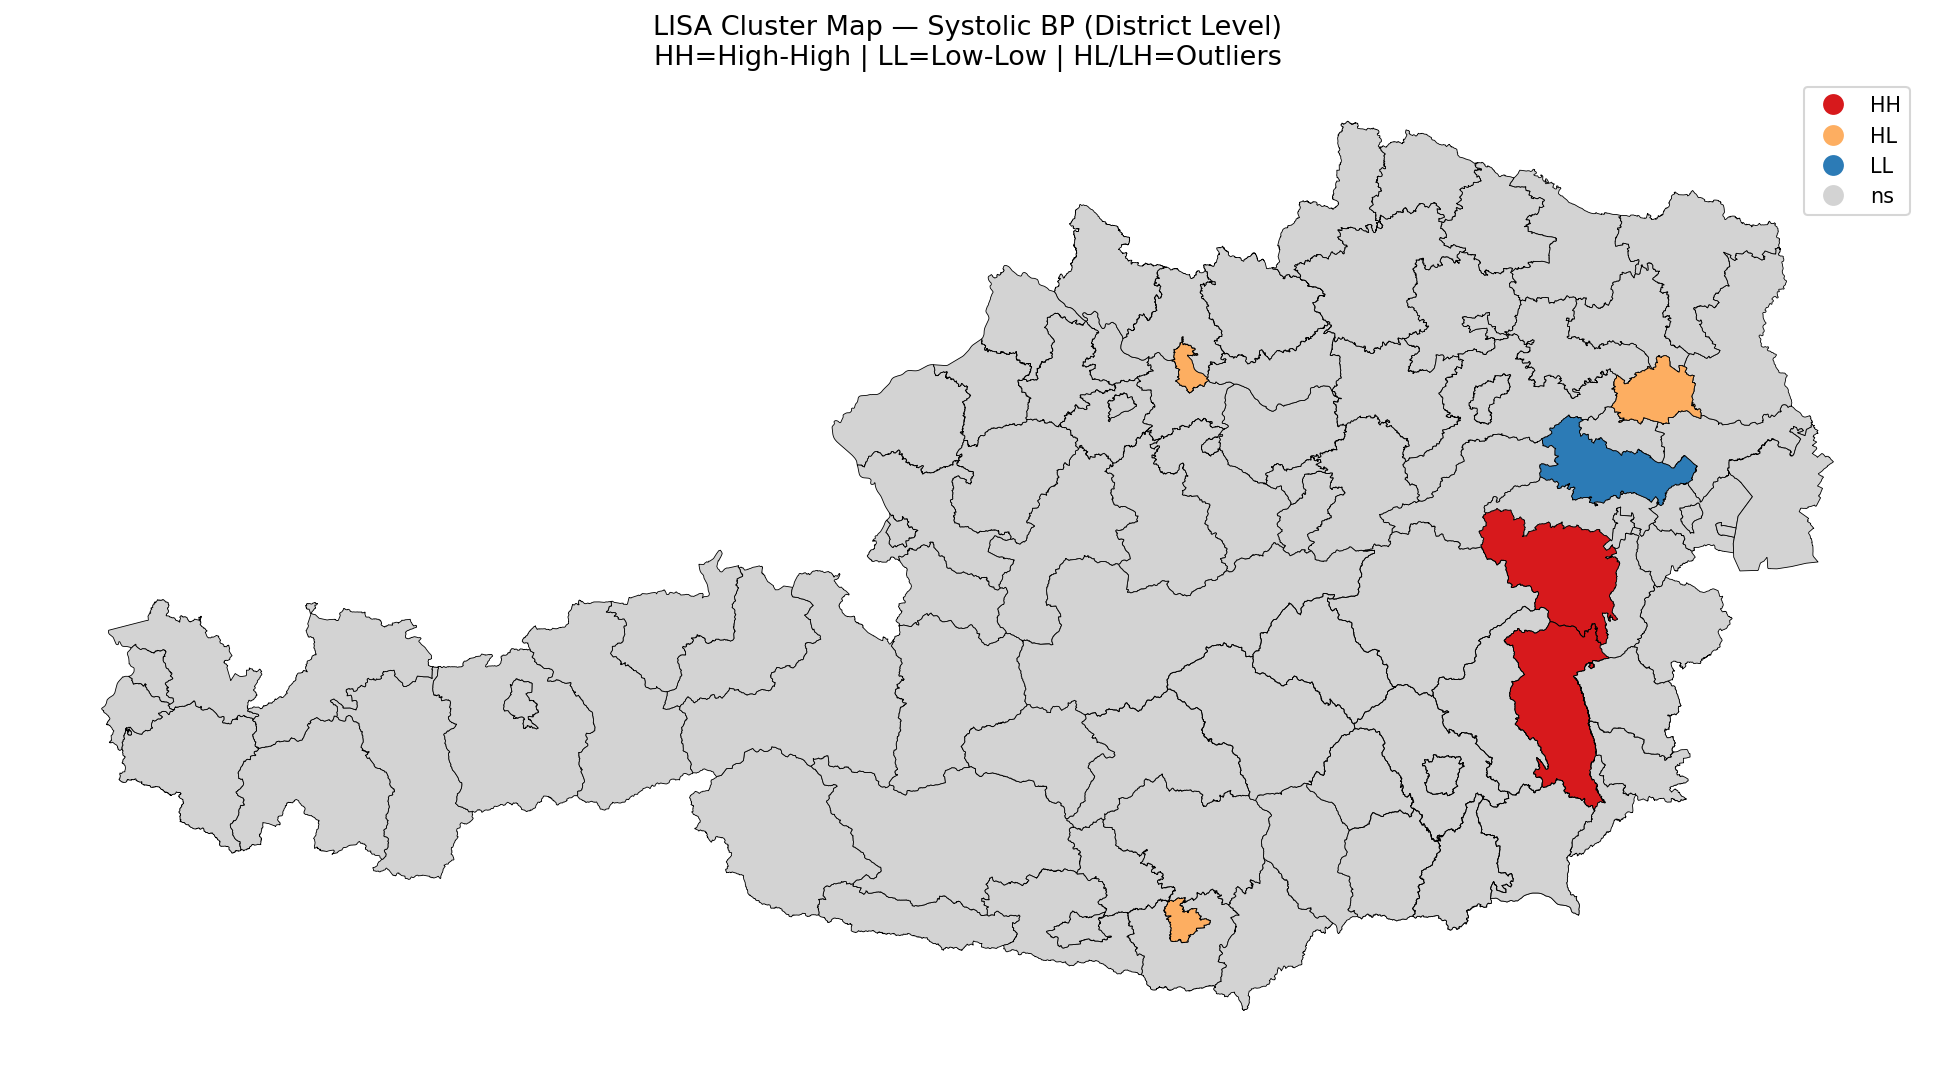
\includegraphics[width=0.9\linewidth, height=0.9\textheight, keepaspectratio]{figures/lisa_clusters_sysbp_district.png}
\end{frame}

\begin{frame}{LISA Cluster Summary --- Key Spatial Findings}

\scriptsize

\begin{columns}[T]

%================ LEFT COLUMN =================
\begin{column}{0.48\textwidth}

\textbf{Hypertension Rate}

\vspace{0.05cm}

\begin{itemize}
\setlength{\itemsep}{0.15em}

\item \textbf{LL Cluster --- Baden}
\begin{itemize}
    \setlength{\itemsep}{0.05em}
    \item Low hypertension surrounded by low neighbouring districts
    \item Stable low-risk zone
\end{itemize}

\item \textbf{HL Urban Outliers}
\begin{itemize}
    \setlength{\itemsep}{0.05em}
    \item Wien, Linz, Klagenfurt
    \item Higher hypertension than surrounding districts
\end{itemize}

\end{itemize}

\end{column}

%================ RIGHT COLUMN =================
\begin{column}{0.48\textwidth}

\textbf{Systolic BP}

\vspace{0.05cm}

\begin{itemize}
\setlength{\itemsep}{0.15em}

\item \textbf{HH Cluster}
\begin{itemize}
    \setlength{\itemsep}{0.05em}
    \item Hartberg-Fürstenfeld \& Neunkirchen
    \item Significant southeastern high-BP cluster
\end{itemize}

\item \textbf{LL Cluster --- Baden}
\begin{itemize}
    \setlength{\itemsep}{0.05em}
    \item Consistent low-BP spatial zone
\end{itemize}

\item \textbf{HL Urban Outliers}
\begin{itemize}
    \setlength{\itemsep}{0.05em}
    \item Wien, Linz, Klagenfurt
\end{itemize}

\end{itemize}

\end{column}

\end{columns}

\vspace{0.5cm}


\small
\textit{Spatial patterns suggest both regional clustering and urban outlier effects in cardiovascular risk.}

\end{frame}



%==================== GDP MAP ====================
\begin{frame}{Regional GDP per Capita (NUTS3) vs BP}
\centering
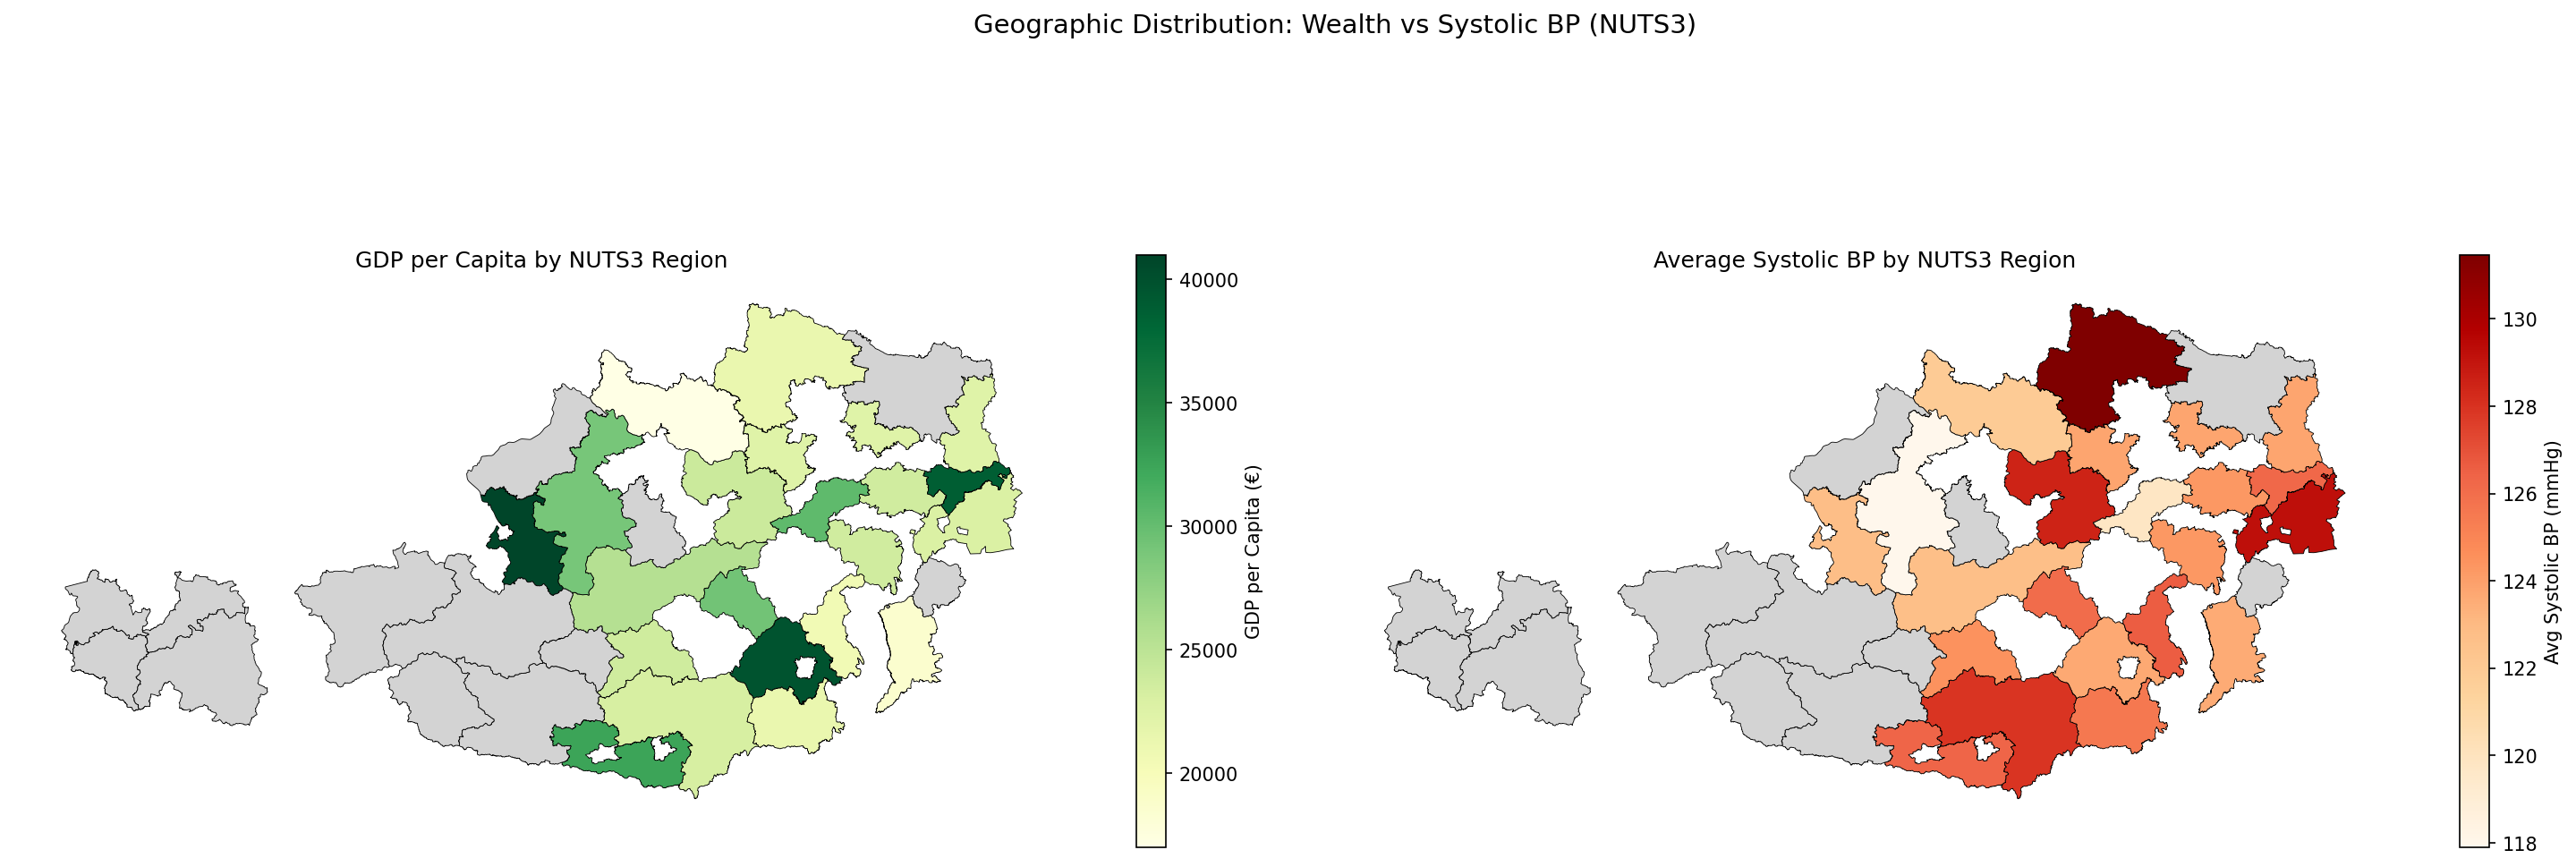
\includegraphics[
    width=0.9\linewidth,
    height=0.85\textheight,
    keepaspectratio
]{figures/nuts3_choropleth_gdp_sysbp.png}
\end{frame}



\begin{frame}{Regional GDP per Capita (NUTS3) vs BP}
\centering
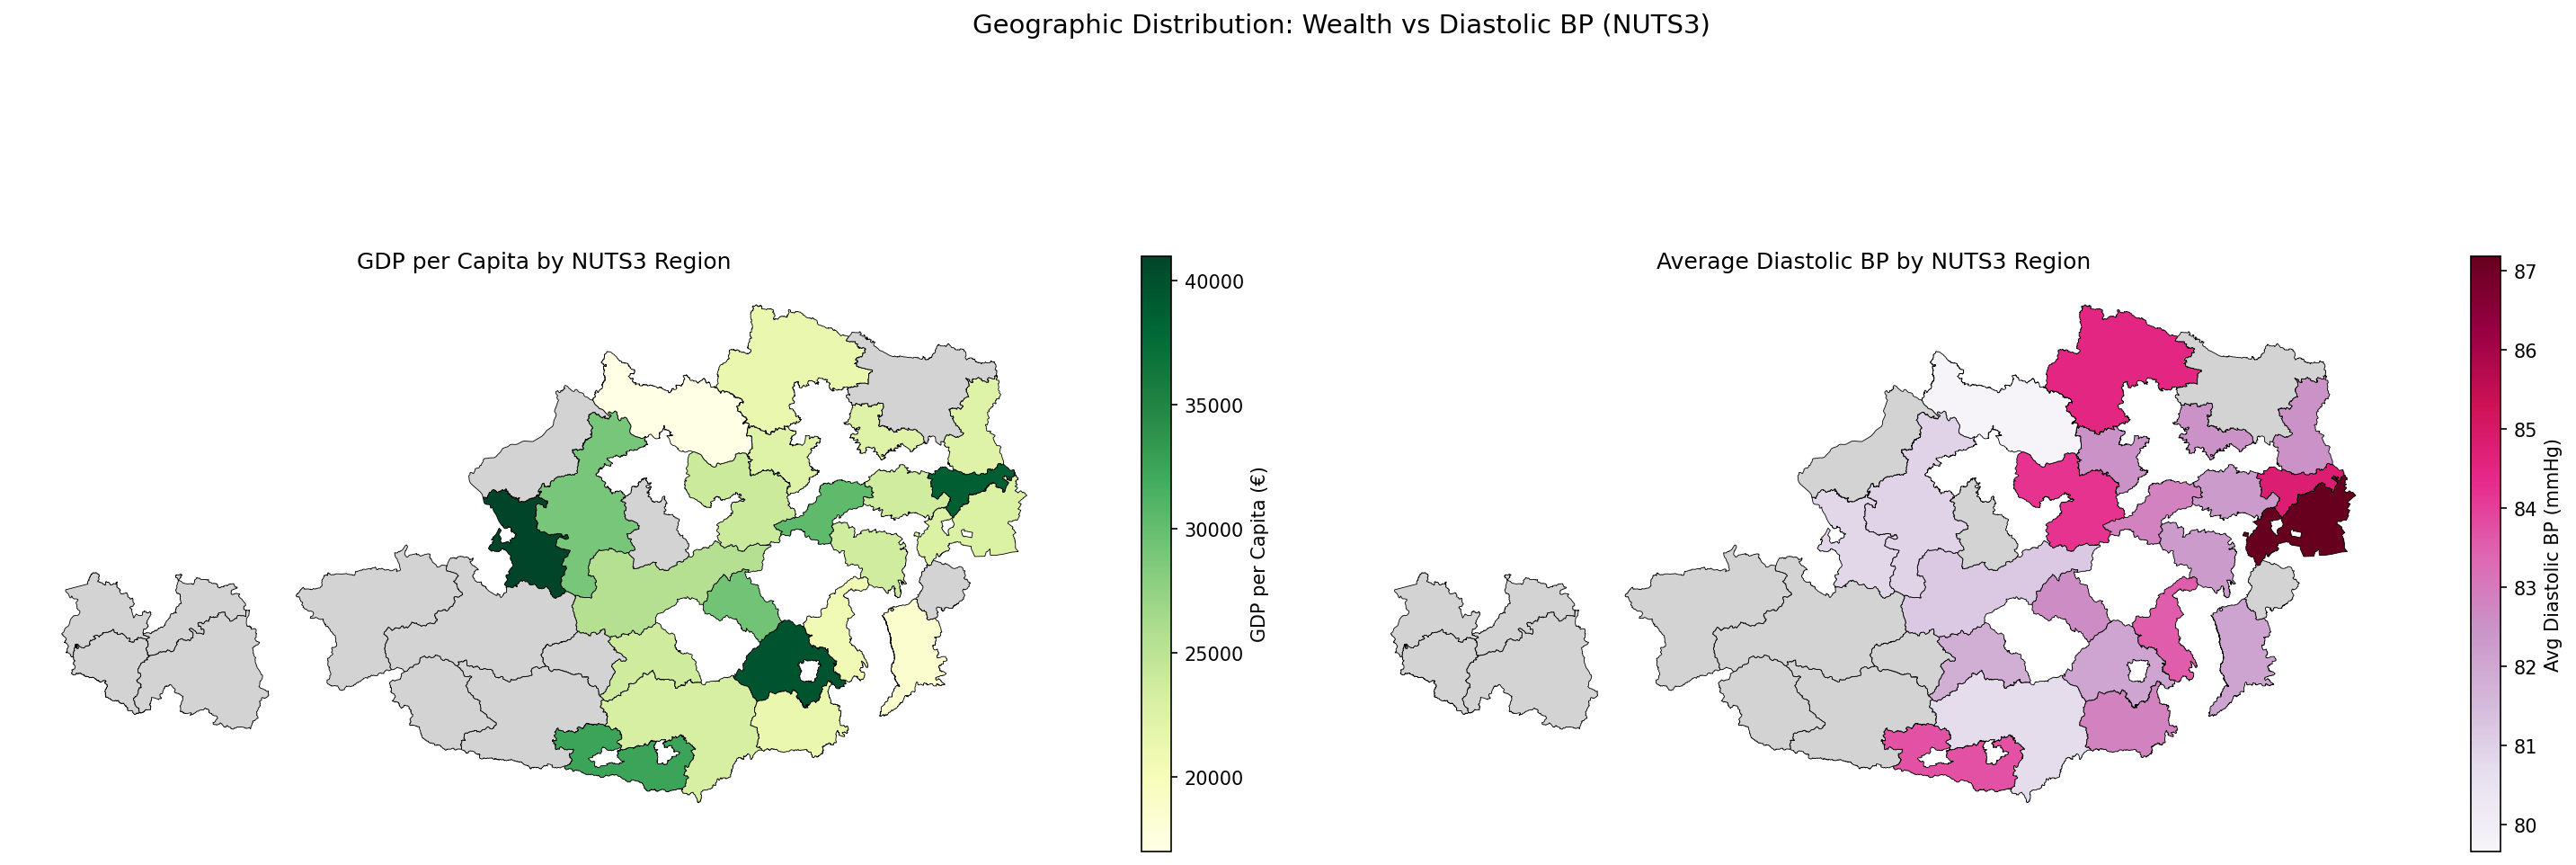
\includegraphics[
    width=0.9\linewidth,
    height=0.85\textheight,
    keepaspectratio
]{figures/nuts3_choropleth_gdp_diabp.png}
\end{frame}


\begin{frame}{Spatial Autocorrelation of Blood Pressure (NUTS3 Level) - GDP}
\centering
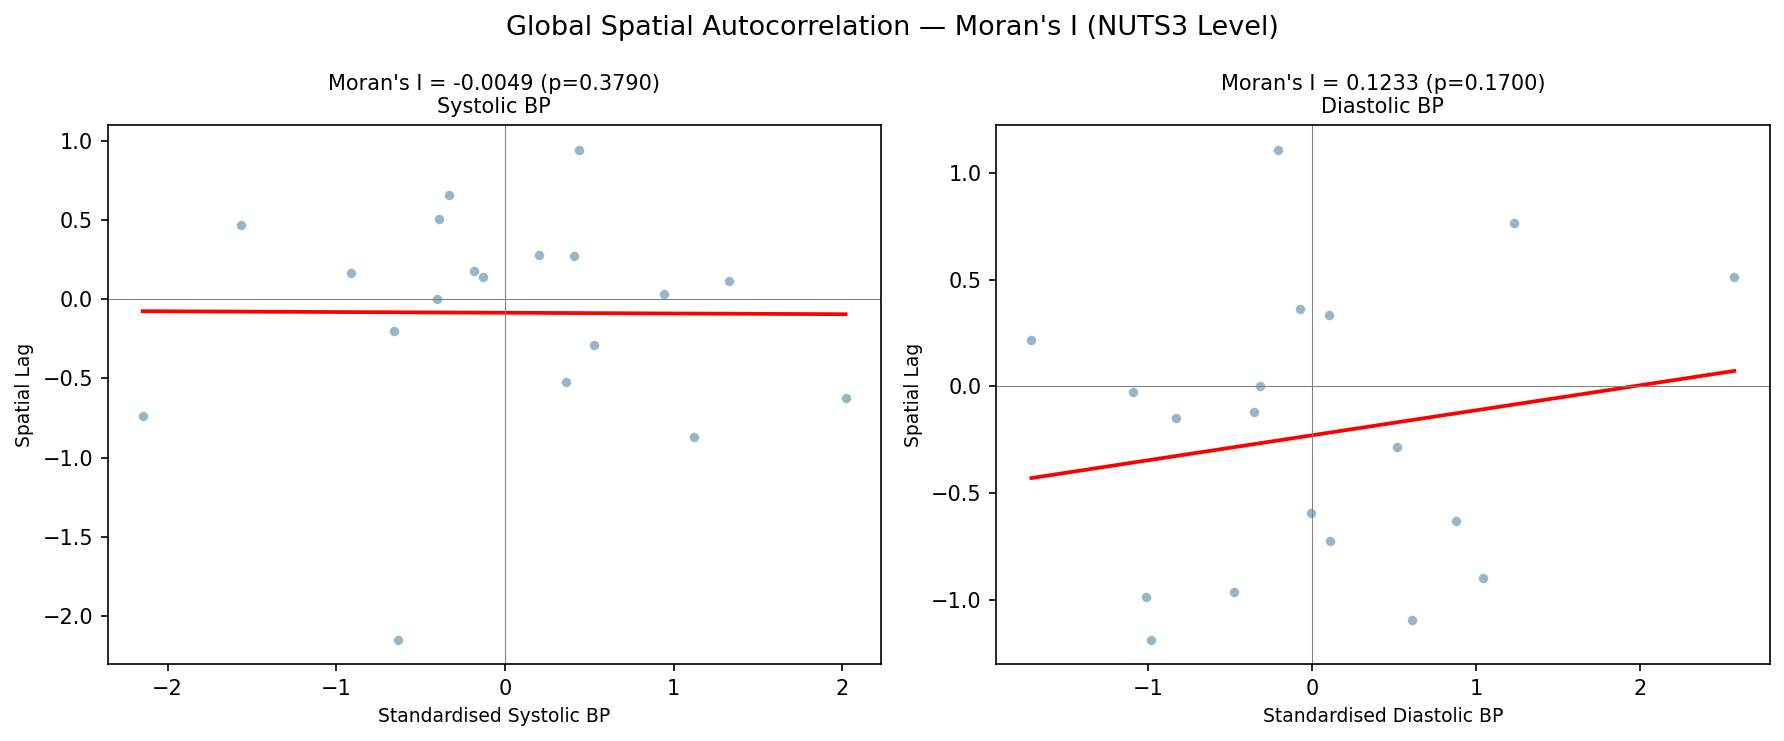
\includegraphics[
    width=0.9\linewidth,
    height=0.85\textheight,
    keepaspectratio
]{figures/morans_I_nuts3.png}
\end{frame}


%==================== GDP SUMMARY ====================
\begin{frame}{GDP and Blood Pressure — Key Findings}

\small

\begin{itemize}

\item Western and central Austrian regions generally showed higher GDP levels with comparatively lower or moderate blood pressure values.

\item Eastern and southeastern regions exhibited higher systolic BP and hypertension prevalence despite mixed economic profiles.

\item Some economically strong urban regions such as Wien and Linz-Wels also showed elevated BP levels, suggesting that higher GDP alone does not protect against cardiovascular risk.

\item Correlation analysis showed only a weak relationship between GDP and systolic BP:
\[
r = -0.064,\quad p = 0.784
\]

\item Spatial autocorrelation at the NUTS3 level was not statistically significant, indicating no strong regional clustering pattern linked to GDP.

\end{itemize}

\end{frame}


%==================== LISA NUTS3 MAP ====================
\begin{frame}{Local Spatial Clusters of Systolic BP (NUTS3 Level)}

\centering

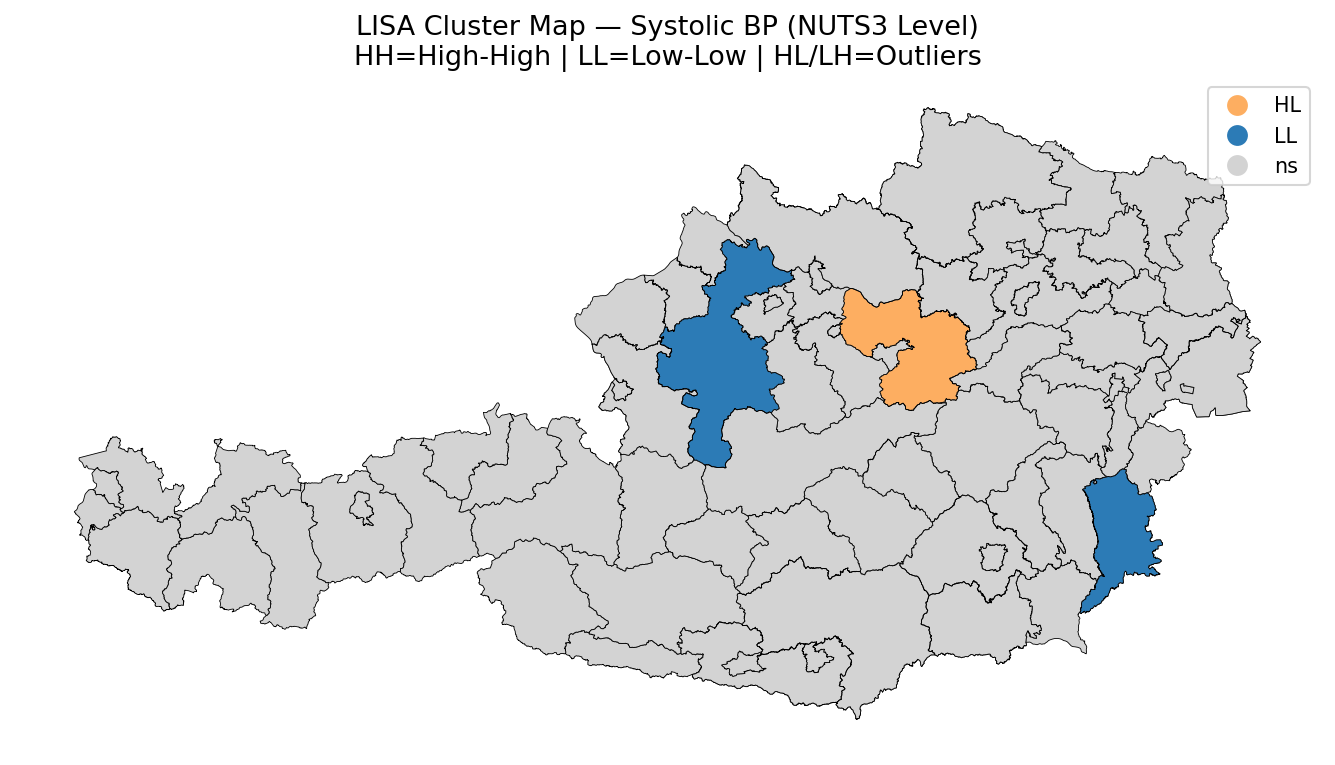
\includegraphics[
    width=0.9\linewidth,
    height=0.85\textheight,
    keepaspectratio
]{figures/lisa_clusters_sysbp_nuts3.png}

\end{frame}


%==================== LISA NUTS3 SUMMARY ====================
\begin{frame}{NUTS3 Spatial Clustering — Key Findings}

\small

\begin{itemize}

\item Although global spatial autocorrelation is not significant at the NUTS3 level , local clustering is still observed.

\item A few regions in central-western and southeastern Austria show Low-Low (LL) BP clusters.

\item Some central and northeastern regions appear as High-Low (HL) outliers, indicating elevated BP relative to neighbouring regions.

\item These findings suggest that BP spatial structure becomes weaker at broader regional aggregation levels compared with district-level analysis.

\end{itemize}

\end{frame}



%==================== CLASSICAL MODELLING ====================
\begin{frame}{Classical Modelling Approach}

\small

\textbf{Method}

\vspace{0.2cm}

\begin{itemize}

\item Ordinary Least Squares (OLS) linear regression.

\item Separate models fitted for:
\begin{itemize}
    \item Mean systolic BP
    \item Mean diastolic BP
\end{itemize}

\item Predictors evaluated using:
\begin{itemize}
    \item Regression coefficient ($\beta$)
    \item p-value (statistical significance)
    \item 95\% confidence interval
\end{itemize}

\item Model performance assessed using 5-fold cross-validation ($R^2$)

\end{itemize}

\vspace{0.25cm}

\footnotesize

\end{frame}


\begin{frame}

\centering
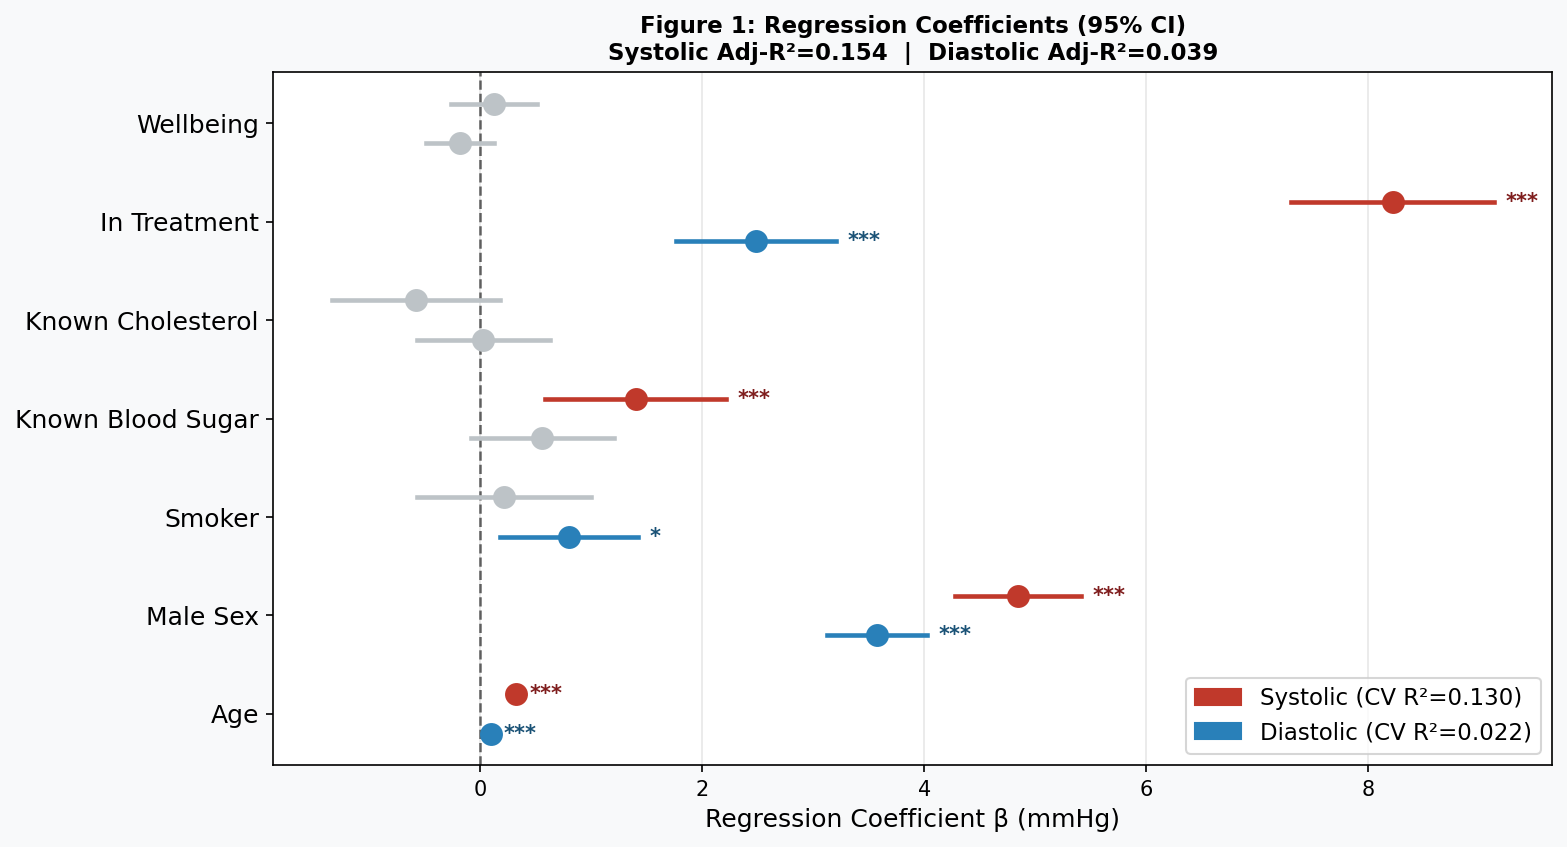
\includegraphics[width=0.9\linewidth, height=0.7\textheight, keepaspectratio]{figures/fig1_forest_plot.png}

\vspace{0.2cm}

\small
\begin{itemize}
    \item Age, Male Sex, and In Treatment are the strongest predictors — all significant. Cholesterol, Wellbeing, and Smoker showed no significant effect on systolic BP.
\end{itemize}

\end{frame} 



\begin{frame}

\centering
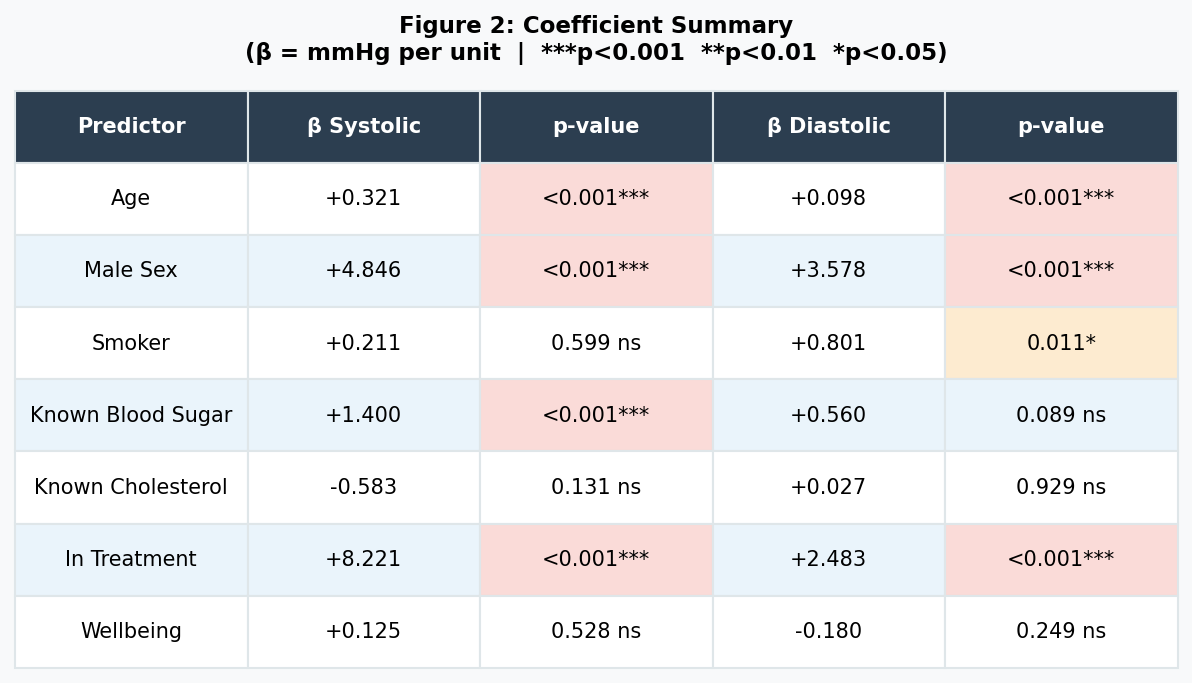
\includegraphics[width=0.9\linewidth, height=0.7\textheight, keepaspectratio]{figures/fig2_coefficient_table.png}

\vspace{0.2cm}

\small
\begin{itemize}
    \item Being in treatment is associated with +8.2 mmHg higher systolic BP. Male sex adds +4.8 mmHg. Every one year of age adds +0.32 mmHg.
\end{itemize}
\end{frame}





\begin{frame}

\centering
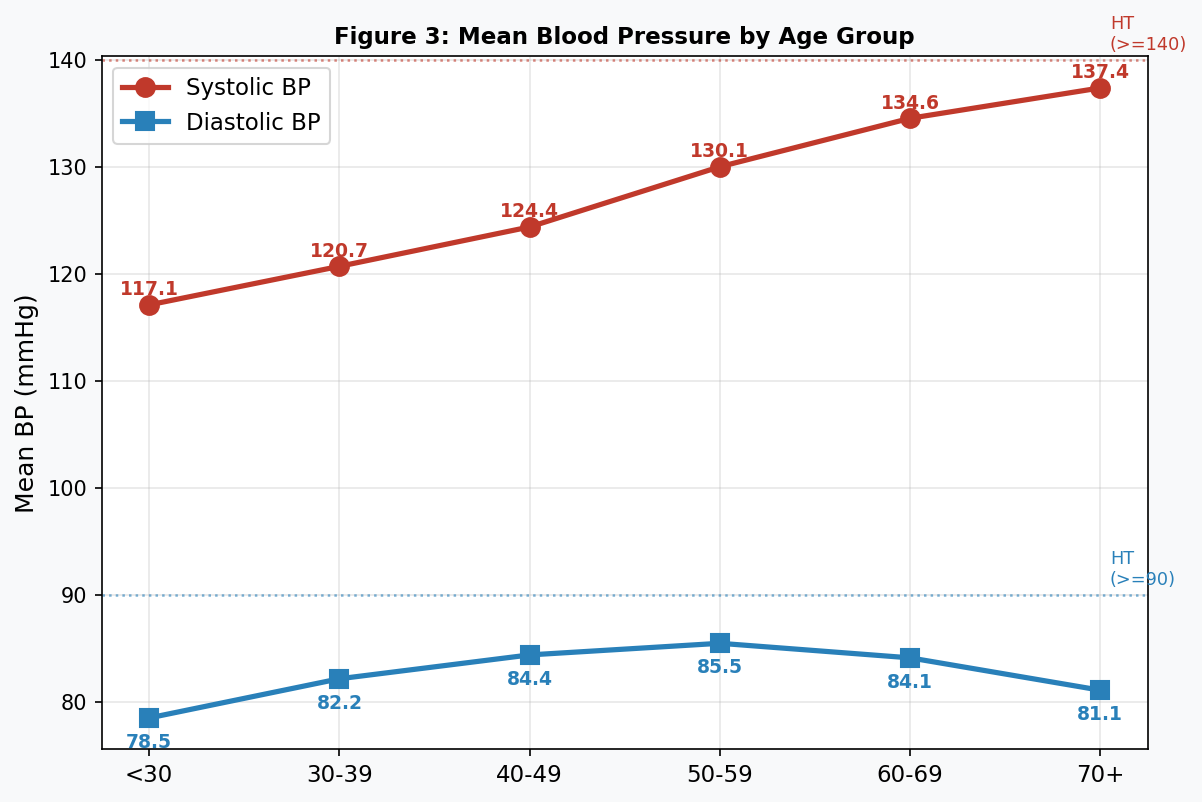
\includegraphics[width=0.9\linewidth, height=0.7\textheight, keepaspectratio]{figures/fig3_bp_by_age_group.png}

\vspace{0.2cm}

\small
\begin{itemize}
    \item systolic BP rises from 117 mmHg in people under 30 to 137 mmHg in people over 70. Diastolic BP peaks around 50 to 59 then slightly drops in older age.
\end{itemize}
\end{frame}



\begin{frame}

\centering
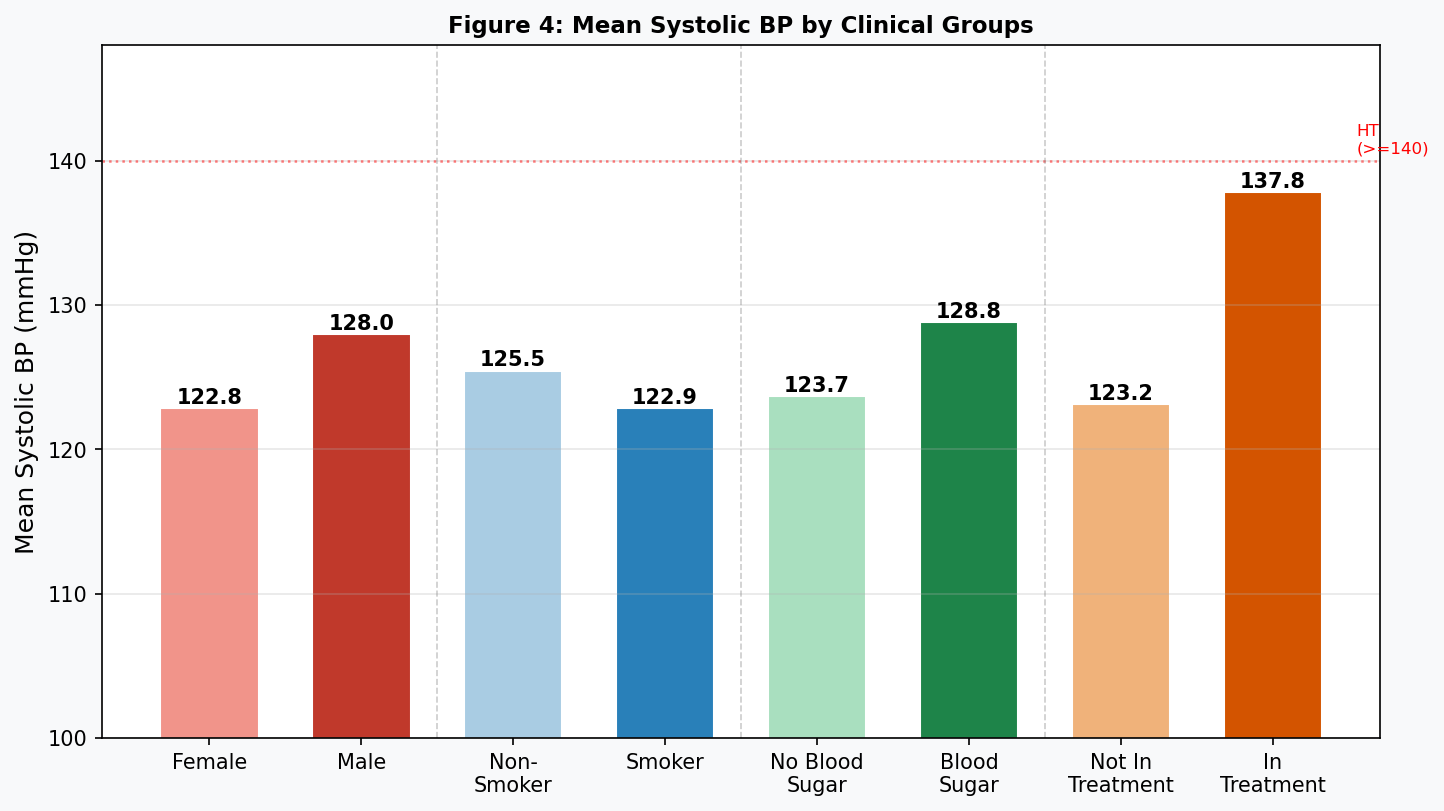
\includegraphics[width=0.9\linewidth, height=0.7\textheight, keepaspectratio]{figures/fig4_bp_by_groups.png}
\end{frame}


\begin{frame}

\centering
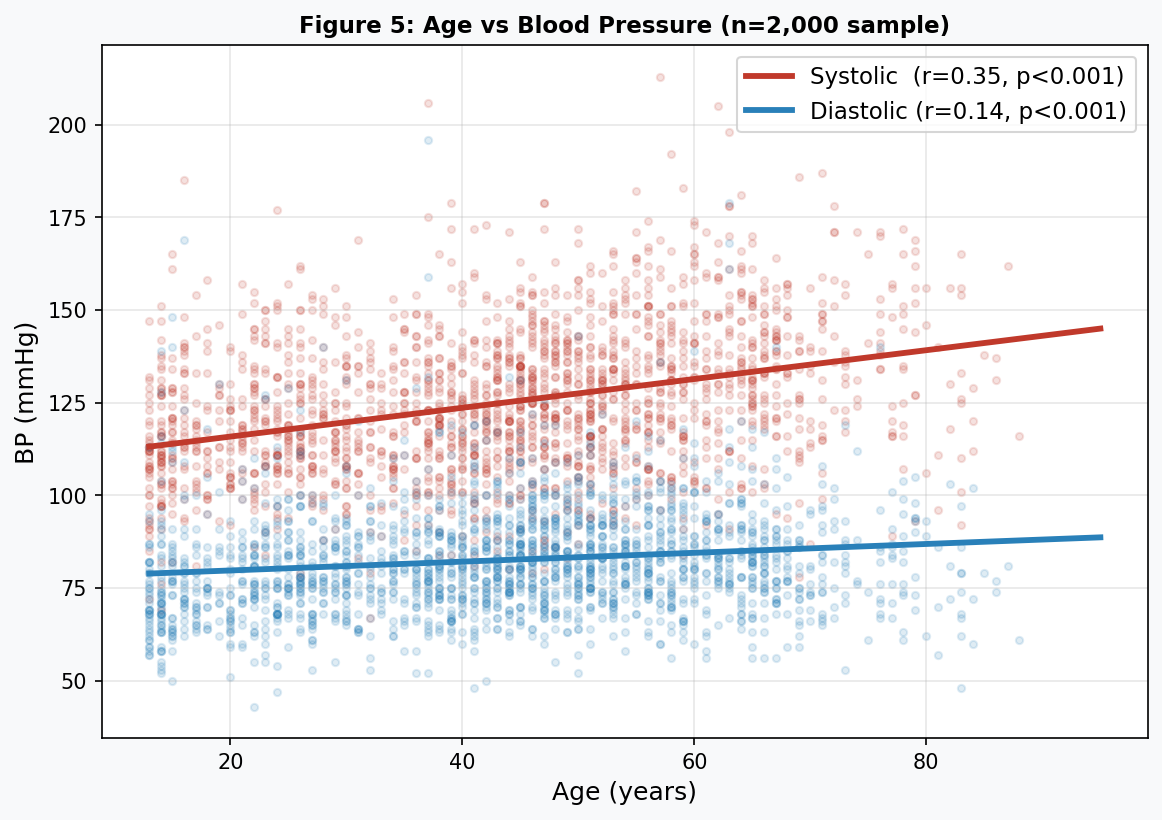
\includegraphics[width=0.9\linewidth, height=0.7\textheight, keepaspectratio]{figures/fig5_age_vs_bp_scatter.png}
\end{frame}


\begin{frame}{Linear Regression —  Summary}

\small
\begin{itemize}
    \item \textbf{Age:} Each additional year increases systolic BP by +0.32 mmHg and diastolic BP by +0.10 mmHg (p<0.001).
    \item \textbf{Sex:} Males have higher BP than females — +4.8 mmHg systolic, +3.6 mmHg diastolic (p<0.001).
    \item \textbf{Treatment Status:} Patients currently in treatment show highest BP — +8.2 mmHg systolic, +2.5 mmHg diastolic (strongest predictor; likely reverse causation).
    \item \textbf{Known Blood Sugar:} Associated with higher systolic BP (+1.4 mmHg); diastolic not significant after adjustment.
    \item \textbf{Smoking:} Increases diastolic BP (+0.80 mmHg, p=0.011); no significant effect on systolic BP.
    \item \textbf{Cholesterol \& Wellbeing:} No significant effect on either BP measure after controlling for other predictors.
\end{itemize}

\end{frame}